%%%========================== %%%
%%%  Set Beamer as class        
%%%==========================%%%
%%
%% Beamer
\documentclass{beamer}
\setbeamercovered{transparent}

%%%========================== %%%
%%%  Set theme        
%%%==========================%%%
%%
%% Warsaw
\usetheme{Warsaw}

%%%========================== %%%
%%%  German Umlauts                            
%%%==========================%%%
%%
%% For Mac OS X
%% \usepackage[applemac]{inputenc}
%% For PC Windows
%% \usepackage[ansinew]{inputenc}
%%
%% For PC Linux 
%% \usepackage[latin1]{inputenc}
%%
%% For UTF-8
\usepackage[utf8]{inputenc}

%%%========================== %%%
%%%  German hyphenation              
%%%==========================%%%
%%
\usepackage{ngerman}

%%%========================== %%%
%%%  Quotes
%%%  \enquote{}       
%%%==========================%%%
%%
\usepackage[babel,german=quotes]{csquotes}

%%%========================== %%%
%%%  Tikz   
%%%==========================%%%
%%
\usepackage{xcolor}
\usepackage{tikz,pgffor}
\usetikzlibrary{shadows}
\tikzset{
	MyPersp/.style={scale=1.8,x={(-0.8cm,-0.4cm)},y={(0.8cm,-0.4cm)},
    z={(0cm,1cm)}},
%  MyPersp/.style={scale=1.5,x={(0cm,0cm)},y={(1cm,0cm)},
%    z={(0cm,1cm)}}, % uncomment the two lines to get a lateral view
	MyPoints/.style={fill=white,draw=black,thick}
		}

% #1 number of teeths
% #2 radius blanket intern
% #3 radius blanket extern
% #4 angle from start to end of the first arc
% #5 angle to decale the second arc from the first 
% #6 radius dna intern
% #7 radius dna extern
% #8 xshift
\newcommand{\gear}[8]{%
  \foreach \i in {1,...,#1} {%
    [rotate=(\i-1)*360/#1]  (0:#2)  arc (0:#4:#2) {[rounded corners=2pt]
     -- (#4+#5:#3)  arc (#4+#5:360/#1-#5:#3)} --  (360/#1:#2)
  }%
  (0,0) circle[radius=#6]
  (0,0) circle[radius=#7];
\draw[thick,xshift=#8]
\foreach \i in {1,2,...,36} {%
  [rotate=(\i-1)*10]  (0.0,#6) -- (0.0,#7)
};
}  

\usepackage{hyperref}


%%%========================== %%%
%%%  Settings for the startpage              
%%%==========================%%%
%%
\title{Introducing: \enquote{The Machine} (DRAFT)}
\author{\texorpdfstring{\ Jürgen Scholz \ \newline\url{j.scholz@machinecoin.org}}{Author}}
\institute{The Machine - A complete self-contained cryptographic ecosphere driven by nothing but the Machinecoin cryptocurrency.}
\date{2014/06/02}

%%%========================== %%%
%%%  Document Start                                
%%%==========================%%%
%%
\begin{document}
\frame{\titlepage}

\frame
{
\tableofcontents
}

\section{Introduction}

\frame
{   
In November 2008, a paper titled ``Bitcoin: A Peer-to-Peer Electronic Cash System'' was posted on The Cryptography Mailing List at metzdowd.com. It was written by either a person or group with the pseudonymous ``Satoshi Nakamoto''. In this paper methods of using a peer-to-peer network to generate a system for electronic transactions without relying on trust were described in detail.
\newline
\newline
\visible<2->{\texttt{``A purely peer-to-peer version of electronic cash would allow online payments to be sent directly from one party to another without going through a financial institution.''}
  \vskip5mm
  \hspace*\fill{\small--- Satoshi Nakamoto, Bitcoin: A Peer-to-Peer Electronic Cash System\footnote{http://bitcoin.org/bitcoin.pdf}}}
}

\frame
{   
In January 2009, these methods came into existence through the release of the first open source Bitcoin client and the issuance of the first bitcoins, with Satoshi Nakamoto, mining the first block of bitcoins, which at this time had a reward of 50 bitcoins. 
\newline
\newline
\visible<2->{In the beginning the values of the first bitcoin transactions were negotiated by individuals on the bitcointalk forums with for example one notable transaction involving a pizza for 10,000 bitcoins\footnote{https://bitcointalk.org/index.php?topic=137.0}.}
\newline
\newline
\visible<3->{These transactions provided a good evidence that it is not just in theory but also in practice possible to have a purely peer-to-peer electronic cash without the need to go through a financial institution.}
}

\frame
{   
Since then a lot of alternative cryptocurrencies have been created. All or most of them are working on the same basis just as Bitcoin does but with slightly different algorithms for special tasks.  
\newline
\newline
\visible<2->{So in general nothing seems to may have changed despite one thing: the major of the cryptoscene has turned cryptocurrencies away from being electronic cash into something that could be better described as classical currency slaves.}
\newline
\newline
\visible<3->{This means that their ``values''\footnote{http://machinecoin.org/wp-content/uploads/2014/04/value.pdf} are rather determined by exchange rates than by real available products or services which a (crypto)currency originally is made for and therefore the cryptoscene has lost the path.}
}

\frame
{
So lets go back to basic and have a look at the primary function of any given (crypto)currency:
\newline
\setbeamercovered{transparent}
\begin{enumerate} 
\item<2-> A (crypto)currency is a medium that makes exchanges of products and/or services between two parties (buyer/seller) possible ...
\item<3-> ... even if the one who is the buyer has got no product and/or service available ...
\item<4-> ... that the seller would like to have and the buyer would like to give in exchange for it
\end{enumerate} 
\ 
\newline
\visible<5->{To focus on this we have decided to model a complete self-contained cryptographic ecosphere driven by nothing but the Machinecoin cryptocurrency.}
}

\frame
{
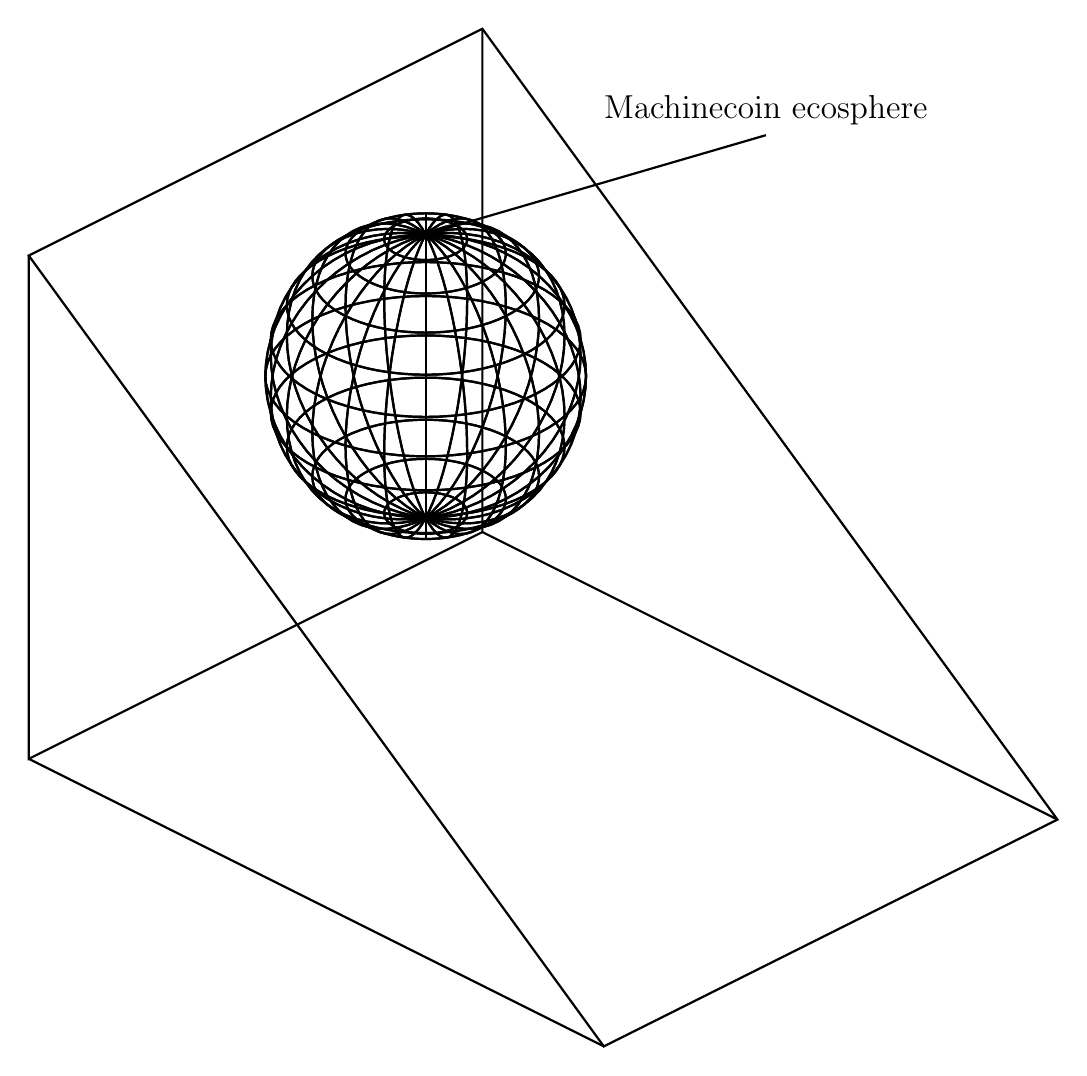
\begin{tikzpicture}[MyPersp,font=\large]
	\def\h{2.5}% Heigth of the ellipse center 
	\def\a{35}% Angle of the section plane with the horizontal
	\def\aa{35}% Angle that defines position of generatrix PA--PB
	\pgfmathparse{\h/tan(\a)}
  	\let\b\pgfmathresult
	\pgfmathparse{sqrt(1/cos(\a)/cos(\a)-1)}
  	\let\c\pgfmathresult %Center Focus distance of the section ellipse.
	\pgfmathparse{\c/sin(\a)}
  	\let\p\pgfmathresult % Position of Dandelin spheres centers
     					% on the Oz axis (\h +/- \p)
	\coordinate (A) at (2,\b,0);
	\coordinate (B) at (-2,\b,0);
	\coordinate (C) at (-2,-1.5,{(1.5+\b)*tan(\a)});
	\coordinate (D) at (2,-1.5,{(1.5+\b)*tan(\a)});
	\coordinate (E) at (2,-1.5,0);
	\coordinate (F) at (-2,-1.5,0);
	\coordinate (CLS) at (0,0,{\h-\p});
	\coordinate (CUS) at (0,0,{\h+\p});
	\coordinate (FA) at (0,{\c*cos(\a)},{-\c*sin(\a)+\h});% Focii
	\coordinate (FB) at (0,{-\c*cos(\a)},{\c*sin(\a)+\h});
	\coordinate (SA) at (0,1,{-tan(\a)+\h}); % Vertices of the
                                           % great axes of the ellipse
	\coordinate (SB) at (0,-1,{tan(\a)+\h});
	\coordinate (PA) at ({sin(\aa},{cos(\aa)},{\h+\p});
	\coordinate (PB) at ({sin(\aa},{cos(\aa)},{\h-\p});
	\coordinate (P) at ({sin(\aa)},{cos(\aa)},{-tan(\a)*cos(\aa)+\h});
     % Point on the ellipse on generatrix PA--PB

	\draw[thick] (A)--(B)--(C)--(D)--cycle;
	\draw[thick] (D)--(E)--(F)--(C);
	\draw[thick] (A)--(E) (B)--(F);


	\foreach \i in {0,0}{%Spheres!
		\foreach \t in {0,15,...,165}% meridians
			{\draw[thick,-] ({cos(\t)},{sin(\t)},\h+\i*\p)
				\foreach \rho in {5,10,...,360}
					{--({cos(\t)*cos(\rho)},{sin(\t)*cos(\rho)},
          {sin(\rho)+\h+\i*\p})}--cycle;
			}
		\foreach \t in {-75,-60,...,75}% parallels
			{\draw[thick,-] ({cos(\t)},0,{sin(\t)+\h+\i*\p})
				\foreach \rho in {5,10,...,360}
					{--({cos(\t)*cos(\rho)},{cos(\t)*sin(\rho)},
          {sin(\t)+\h+\i*\p})}--cycle;
			}
		}

    \draw[thick,-] (17.5,17.5,17.5) -- (17,20,19) node[right,above]{Machinecoin ecosphere};
\end{tikzpicture}
}


%\section{Bibliography}
%\begin{frame}
%	\frametitle{Quellen}
%	\bibliographystyle{alpha}
%	\bibliography{literatur}		
%\end{frame} 

\end{document}
%%%%%%%%%%%%%%%%%%%%%%
%%%  Dokument Ende                           
%%%%%%%%%%%%%%%%%%%%%%